% ======================================================================
% Projeto de Graduação em Computação (PGC) — UFABC
% Pedido de Orientação de PGC I
% Tema: Iridologia sob Lentes Científicas — Avaliação Crítica com
%       Aprendizado de Máquina (ênfase em biomarcadores médicos da íris para DM2)
% ======================================================================

\documentclass[12pt,a4paper]{article}

% ---------------------- Pacotes ----------------------
\usepackage[utf8]{inputenc}
\usepackage[T1]{fontenc}
\usepackage{lmodern}
\usepackage[portuguese]{babel}

\usepackage{setspace}
\usepackage{geometry}
\geometry{a4paper, top=3cm, bottom=2.5cm, left=3cm, right=2.5cm}

\usepackage{graphicx}
\graphicspath{{./imagens/}}
\usepackage{float}

\usepackage{amsmath, amssymb}
\usepackage{siunitx}
\sisetup{
  mode = match,
  propagate-math-font = true,
  reset-math-version = false,
  reset-text-family = false,
  reset-text-series = false,
  reset-text-shape = false,
  text-family-to-math = true,
  text-series-to-math = true
}

\usepackage{booktabs}
\usepackage{multirow}
\usepackage{array}
\usepackage{tabularx}
\usepackage{xcolor}

\usepackage{fancyhdr}
\setlength{\headheight}{14pt}

% Natbib em autor--ano (compatível com \bibitem[Autor(ano)]{...})
\usepackage[authoryear, round, sort]{natbib}

% hyperref por último (boa prática)
\usepackage[bookmarks=true, colorlinks=true, linkcolor=blue, citecolor=blue, urlcolor=blue]{hyperref}

\usepackage{indentfirst}
\setlength{\parindent}{1.25cm}
\setlength{\parskip}{0.2cm}

% TikZ / pgfplots para figuras vetoriais
\usepackage{tikz}
\usetikzlibrary{arrows.meta, positioning, calc, shapes.geometric, backgrounds, fit}
\usepackage{pgfplots}
\pgfplotsset{compat=1.18}

% ---------------------- Cabeçalho/Rodapé ----------------------
\pagestyle{fancy}
\fancyhf{}
\lhead{\small UFABC --- Projeto de Graduação em Computação}
\rhead{\small Pedido de Orientação --- PGC I}
\cfoot{\thepage}

% ----------------------------------------------------------------------
\begin{document}

\hypersetup{pageanchor=false}

% ====================== Capa ======================
\begin{titlepage}
\begin{center}

{\large \textbf{UNIVERSIDADE FEDERAL DO ABC}}\\[0.25cm]
{\large \textbf{BACHARELADO EM CIÊNCIA DA COMPUTAÇÃO}}\\[0.25cm]
{\large \textbf{PROJETO DE GRADUAÇÃO EM COMPUTAÇÃO (PGC)}}\\[1.2cm]

\rule{\textwidth}{0.4pt}\\[0.4cm]
{\LARGE \textbf{Iridologia sob Lentes Científicas:}}\\[0.2cm]
{\Large \textbf{Avaliação Crítica com Aprendizado de Máquina}}\\[0.3cm]
{\large \textit{Da hipótese iridológica aos biomarcadores médicos da íris:\\
vascularização, diâmetro pupilar e morfologia para inferência de DM2}}\\[0.3cm]
\rule{\textwidth}{0.4pt}\\[1.2cm]

\vfill
{\normalsize Santo André --- SP}\\
{\normalsize \today}

\end{center}
\end{titlepage}

% ====================== Resumo ======================
\begin{abstract}
\noindent
Este Projeto de Graduação em Computação (PGC) investiga se fotografias convencionais da íris permitem
estimar alterações oculares associadas ao diabetes mellitus tipo~2 (DM2) com técnicas de visão
computacional e aprendizado de máquina. O trabalho não utiliza mapas da iridologia, prática sem
respaldo clínico. A análise se concentra em grandezas estudadas na literatura médica: vascularização
da íris, diâmetro pupilar e morfologia iridiana e pupilar. Estudos com AS-OCTA relatam redução da
densidade vascular da íris em pessoas com DM2 \citep{Zhou2025SciRep} e mostram que essa modalidade
permite visualizar a vasculatura iridiana \citep{Roberts2017CER,Zett2018Graefes}. Outros trabalhos
descrevem alterações no diâmetro pupilar e na espessura da íris
\citep{Cui2024BMC,Thakar2025Eye}.

Foi reimplementado um fluxo computacional que inclui segmentação de íris e pupila, normalização
geométrica \emph{rubber sheet}, extração de descritores de intensidade, \textit{Local Binary
Patterns} e Haralick e validação cruzada estratificada por grupos. A avaliação por pessoa depende de
identificadores reais. Como a base legada não contém esses identificadores e não permite confirmar
que a classe positiva corresponde especificamente a DM2, seus resultados são apresentados somente
como uma análise provisória dos rótulos fornecidos.

O projeto também define o conjunto de metadados necessário para uma avaliação clínica, incorpora
ResNet, EfficientNet e \emph{Vision Transformers}, acrescenta descritores morfológicos e cromáticos e
mede correlatos de vascularização em imagens RGB. Esses correlatos não substituem medidas obtidas por
AS-OCTA. O objetivo desta etapa é verificar a viabilidade e a estabilidade das medidas, controlar
fontes de viés e registrar as condições necessárias para uma avaliação posterior com dados clínicos
verificáveis.

\vspace{0.3cm}
\noindent\textbf{Palavras-chave:} diabetes mellitus tipo 2; íris; vascularização; diâmetro pupilar;
visão computacional; aprendizado de máquina; aprendizado profundo; biomarcadores oculares.
\end{abstract}

\tableofcontents
\newpage

\hypersetup{pageanchor=true}
\pagenumbering{arabic}
\setcounter{page}{1}

\onehalfspacing

% ====================== Introdução ======================
\section{Introdução}

A textura da íris permite distinguir indivíduos e é utilizada em sistemas biométricos
\citep{Daugman2004}. A íris também contém vasos e os músculos responsáveis pelo controle do diâmetro
pupilar. Essas características aparecem tanto em estudos médicos sobre manifestações oculares de
doenças sistêmicas quanto em práticas sem respaldo científico, como a \emph{iridologia}.

A iridologia sustenta que regiões da íris se mapeariam topograficamente a órgãos e sistemas, de modo
que alterações locais refletiriam disfunções internas. Quando avaliada sob protocolos controlados, no
entanto, a prática apresenta baixa acurácia e confiabilidade diagnóstica \citep{Simon1979JAMA,
Ernst2000ArchOphthalmol}. Em uma etapa preliminar deste projeto, utilizou-se código legado para testar
se imagens da íris conteriam \emph{sinal estatístico} associado ao diabetes. A auditoria posterior do
material identificou 73 linhas duplicadas entre 196 amostras e ausência de identificadores reais de
indivíduo. Assim, o resultado histórico de acurácia próxima de 0,92 não constitui evidência de
particionamento por pessoa nem de associação específica com DM2. Essa constatação motivou a
reimplementação do código, com deduplicação, registro dos \textit{folds}, múltiplas
métricas e bloqueios explícitos quando identidade e diagnóstico não podem ser verificados.

Por essa razão, este PGC não procura confirmar mapas iridológicos. O objeto de estudo são medidas
oculares presentes na literatura clínica sobre DM2: vascularização da íris, diâmetro pupilar,
espessura e morfologia iridianas. A distinção é importante porque essas medidas podem ser definidas e
comparadas, enquanto as associações topográficas propostas pela iridologia não encontram suporte em
avaliações controladas.

Estudos com angiografia por tomografia de coerência óptica do segmento anterior (AS-OCTA) relatam
redução da densidade vascular da íris em pessoas com DM2, inclusive sem retinopatia diabética
\citep{Zhou2025SciRep}, e avaliam a identificação da vasculatura iridiana
\citep{Roberts2017CER,Zett2018Graefes}. Também há relatos de alterações no diâmetro pupilar e na
espessura da íris \citep{Cui2024BMC,Thakar2025Eye}. A partir desses resultados, o projeto pergunta se
fotografias convencionais contêm correlatos mensuráveis dessas grandezas, ainda que sem a informação
vascular fornecida pela AS-OCTA.

O estudo é exploratório. Ele examina a viabilidade técnica dessas medidas, sua sensibilidade às
condições de aquisição e o desempenho dos classificadores sob um protocolo reproduzível. O arquivo
legado serve apenas para validar a execução e produzir uma análise provisória. Conclusões sobre DM2 e
generalização por pessoa dependem de rótulos clínicos verificáveis, identificadores reais e validação
em um conjunto independente.

% ====================== Problema ======================
\section{Problema e Questões de Pesquisa}

\subsection{Contexto e motivação}
A literatura clínica clássica não sustenta a iridologia como método diagnóstico
\citep{Simon1979JAMA,Ernst2000ArchOphthalmol}. Por outro lado, a medicina reconhece que o olho ---
incluindo o segmento anterior --- pode manifestar repercussões sistêmicas do DM2. A microangiopatia
diabética, por exemplo, não se restringe à retina: estudos com AS-OCTA evidenciam rarefação vascular
na íris \citep{Zhou2025SciRep}, enquanto disautonomia diabética afeta a dinâmica pupilar
\citep{Thakar2025Eye}. Surge, então, uma oportunidade de pesquisa distinta da iridologia: investigar
se \textbf{grandezas oculares clinicamente reconhecidas} associadas ao DM2 podem ser \emph{aproximadas}
a partir de imagens convencionais por visão computacional, e se tais aproximações carregam sinal útil.

A avaliação deve verificar se o desempenho observado é reprodutível, permanece estável entre
reamostragens, não decorre de artefatos de aquisição ou vazamento de dados e admite interpretação
compatível com as medidas oculares investigadas. O particionamento por pessoa só pode ser avaliado
quando houver identificadores reais.

\subsection{Problema central}
\emph{É viável aproximar, a partir de fotografias convencionais da íris e por meio de visão
computacional e aprendizado de máquina, biomarcadores oculares clinicamente associados ao DM2 ---
vascularização, diâmetro pupilar e morfologia iridiana --- de modo reprodutível, generalizável e
controlado contra viés?}

\subsection{Questões específicas}
\begin{enumerate}
    \item \textbf{Viabilidade de extração de medidas oculares.} É possível extrair, de imagens
    RGB, correlatos confiáveis de (a)~vascularização/textura vascular, (b)~diâmetro pupilar e
    geometria da coroa pupilar, e (c)~morfologia iridiana (criptas, sulcos, colarete), apesar das
    limitações de fotografias não obtidas por AS-OCTA?

    \item \textbf{Validade e estabilidade do sinal.} Em um conjunto com diagnóstico de DM2 e
    identificadores reais, o desempenho preditivo permanece consistente entre \textit{folds},
    sementes e perturbações fotométricas quando o particionamento é feito por pessoa?

    \item \textbf{Contribuição das arquiteturas profundas.} Arquiteturas como ResNet, EfficientNet e
    \emph{Vision Transformers}, sob \emph{transfer learning} e particionamento por pessoa,
    agregam capacidade discriminativa real em relação à linha de base clássica, ou apenas ampliam o
    risco de sobreajuste e de captura de artefatos?

    \item \textbf{Interpretabilidade morfológica e cromática.} Descritores morfológicos (desvios em
    relação à circunferência ajustada, estruturas locais) e cromáticos (HSV e LAB) fornecem ganho
    consistente e clinicamente plausível, ou se comportam como ruído sob múltiplas comparações?
\end{enumerate}

% ====================== Objetivos ======================
\section{Objetivos}

\subsection{Objetivo geral}
Investigar se fotografias convencionais da íris permitem estimar correlatos de vascularização,
diâmetro pupilar e morfologia iridiana e pupilar associados ao DM2, utilizando visão computacional e
aprendizado de máquina. A avaliação deve controlar fontes de viés e vazamento de dados e medir a
capacidade de generalização.

\subsection{Objetivos específicos}
\begin{itemize}
    \item \textbf{Revisão médica e computacional.} Sintetizar a evidência clínica sobre alterações
    oculares do segmento anterior no DM2 (vascularização, diâmetro pupilar, espessura/morfologia) e os
    métodos de visão computacional aplicáveis à extração dessas grandezas a partir de imagens RGB.

    \item \textbf{Estudo de viabilidade das medidas oculares.} Implementar e avaliar técnicas de
    visão computacional para estimar correlatos de vascularização (realce e densidade de estruturas
    vasculares/texturais), diâmetro pupilar e geometria da coroa pupilar, documentando limites e
    incertezas dessas estimativas em imagens convencionais.

    \item \textbf{Eixo 1 --- Base de trabalho e proveniência clínica.} Consolidar uma base com rótulo
    clínico de DM2 verificável, identificador real de indivíduo, lateralidade e fonte do diagnóstico.
    Enquanto esses metadados não estiverem disponíveis, restringir o arquivo legado à validação
    operacional e à análise exploratória de rótulos reportados, sem alegar particionamento por pessoa.

    \item \textbf{Eixo 2 --- Arquiteturas profundas.} Incorporar ResNet, EfficientNet e \emph{Vision
    Transformers} sob \emph{transfer learning} e, após a obtenção dos identificadores reais,
    particionamento por pessoa, comparando-as com a linha de base clássica sob as mesmas divisões.

    \item \textbf{Eixo 3 --- Caracterização morfológica.} Quantificar a morfologia da íris e da coroa
    pupilar por meio de desvios em relação à circunferência ajustada e da identificação de estruturas
    (criptas, sulcos, colaretes), conectando-as ao diâmetro pupilar.

    \item \textbf{Eixo 4 --- Descritores cromáticos.} Introduzir descritores baseados em momentos de
    cor e histogramas regionais nos espaços HSV e LAB, avaliando seu ganho marginal sobre os
    descritores existentes.

    \item \textbf{Integração e avaliação crítica.} Integrar as extensões ao fluxo computacional,
    permitindo comparações diretas com múltiplas métricas (acurácia, sensibilidade,
    especificidade, precisão e F1) e análises de estabilidade (reamostragens, \textit{folds} e
    sementes).
\end{itemize}

% ====================== Fundamentação ======================
\section{Fundamentação Teórica}

\subsection{Anatomia do segmento anterior e a íris}
A íris é o diafragma colorido do olho, situado no segmento anterior, entre a córnea e o cristalino
(Figura~\ref{fig:olho-anatomia}). Ela separa as câmaras anterior e posterior e controla a quantidade
de luz que atinge a retina por meio da pupila, cujo diâmetro é regulado por dois músculos antagonistas:
o esfíncter da pupila (constrição/miose) e o dilatador (dilatação/midríase). A íris é vascularizada
pelo \emph{círculo arterial maior} e por ramos radiais que convergem em direção à pupila, e sua
superfície anterior exibe estruturas características --- criptas, sulcos de contração e o
\emph{colarete} (ou coroa) --- relevantes tanto para biometria \citep{Daugman2004} quanto para a
caracterização morfológica proposta neste projeto.

\begin{figure}[H]
    \centering
    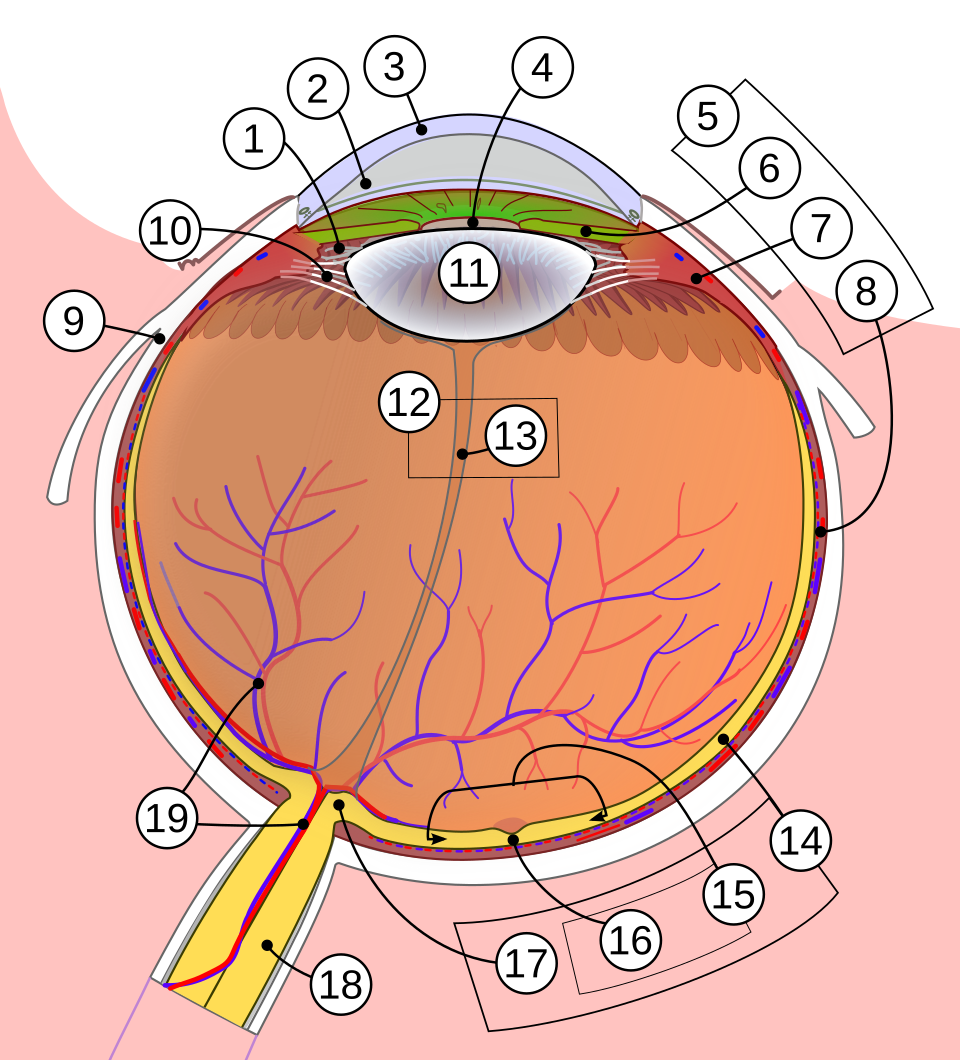
\includegraphics[width=0.72\textwidth]{olho_anatomia.png}
    \caption{Corte esquemático do olho humano. Estruturas de interesse direto para este projeto
    situam-se no segmento anterior: \textbf{6~--~íris}, \textbf{4~--~pupila}, \textbf{2~--~câmara
    anterior} e \textbf{3~--~córnea}. Diagrama de Rhcastilhos, editado por User:Jakov, em domínio
    público via Wikimedia Commons.}
    \label{fig:olho-anatomia}
\end{figure}

\subsection{Morfologia da íris e a coroa pupilar}
A Figura~\ref{fig:iris-closeup} apresenta uma macrofotografia da íris na qual se observam o padrão
radial de fibras (trabéculas), criptas e o colarete --- a faixa sinuosa que delimita a zona pupilar
(interna) da zona ciliar (externa). Essas estruturas constituem o substrato visual da
\textbf{caracterização morfológica} (Eixo~3): desvios da borda pupilar em relação a uma circunferência
ajustada, ondulações do colarete e densidade de criptas são candidatos a descritores quantitativos.
Do ponto de vista médico, a geometria da coroa pupilar e a regularidade da borda pupilar relacionam-se
ao tônus muscular e, indiretamente, à integridade da inervação autonômica, frequentemente comprometida
no DM2 \citep{Thakar2025Eye}.

\begin{figure}[H]
    \centering
    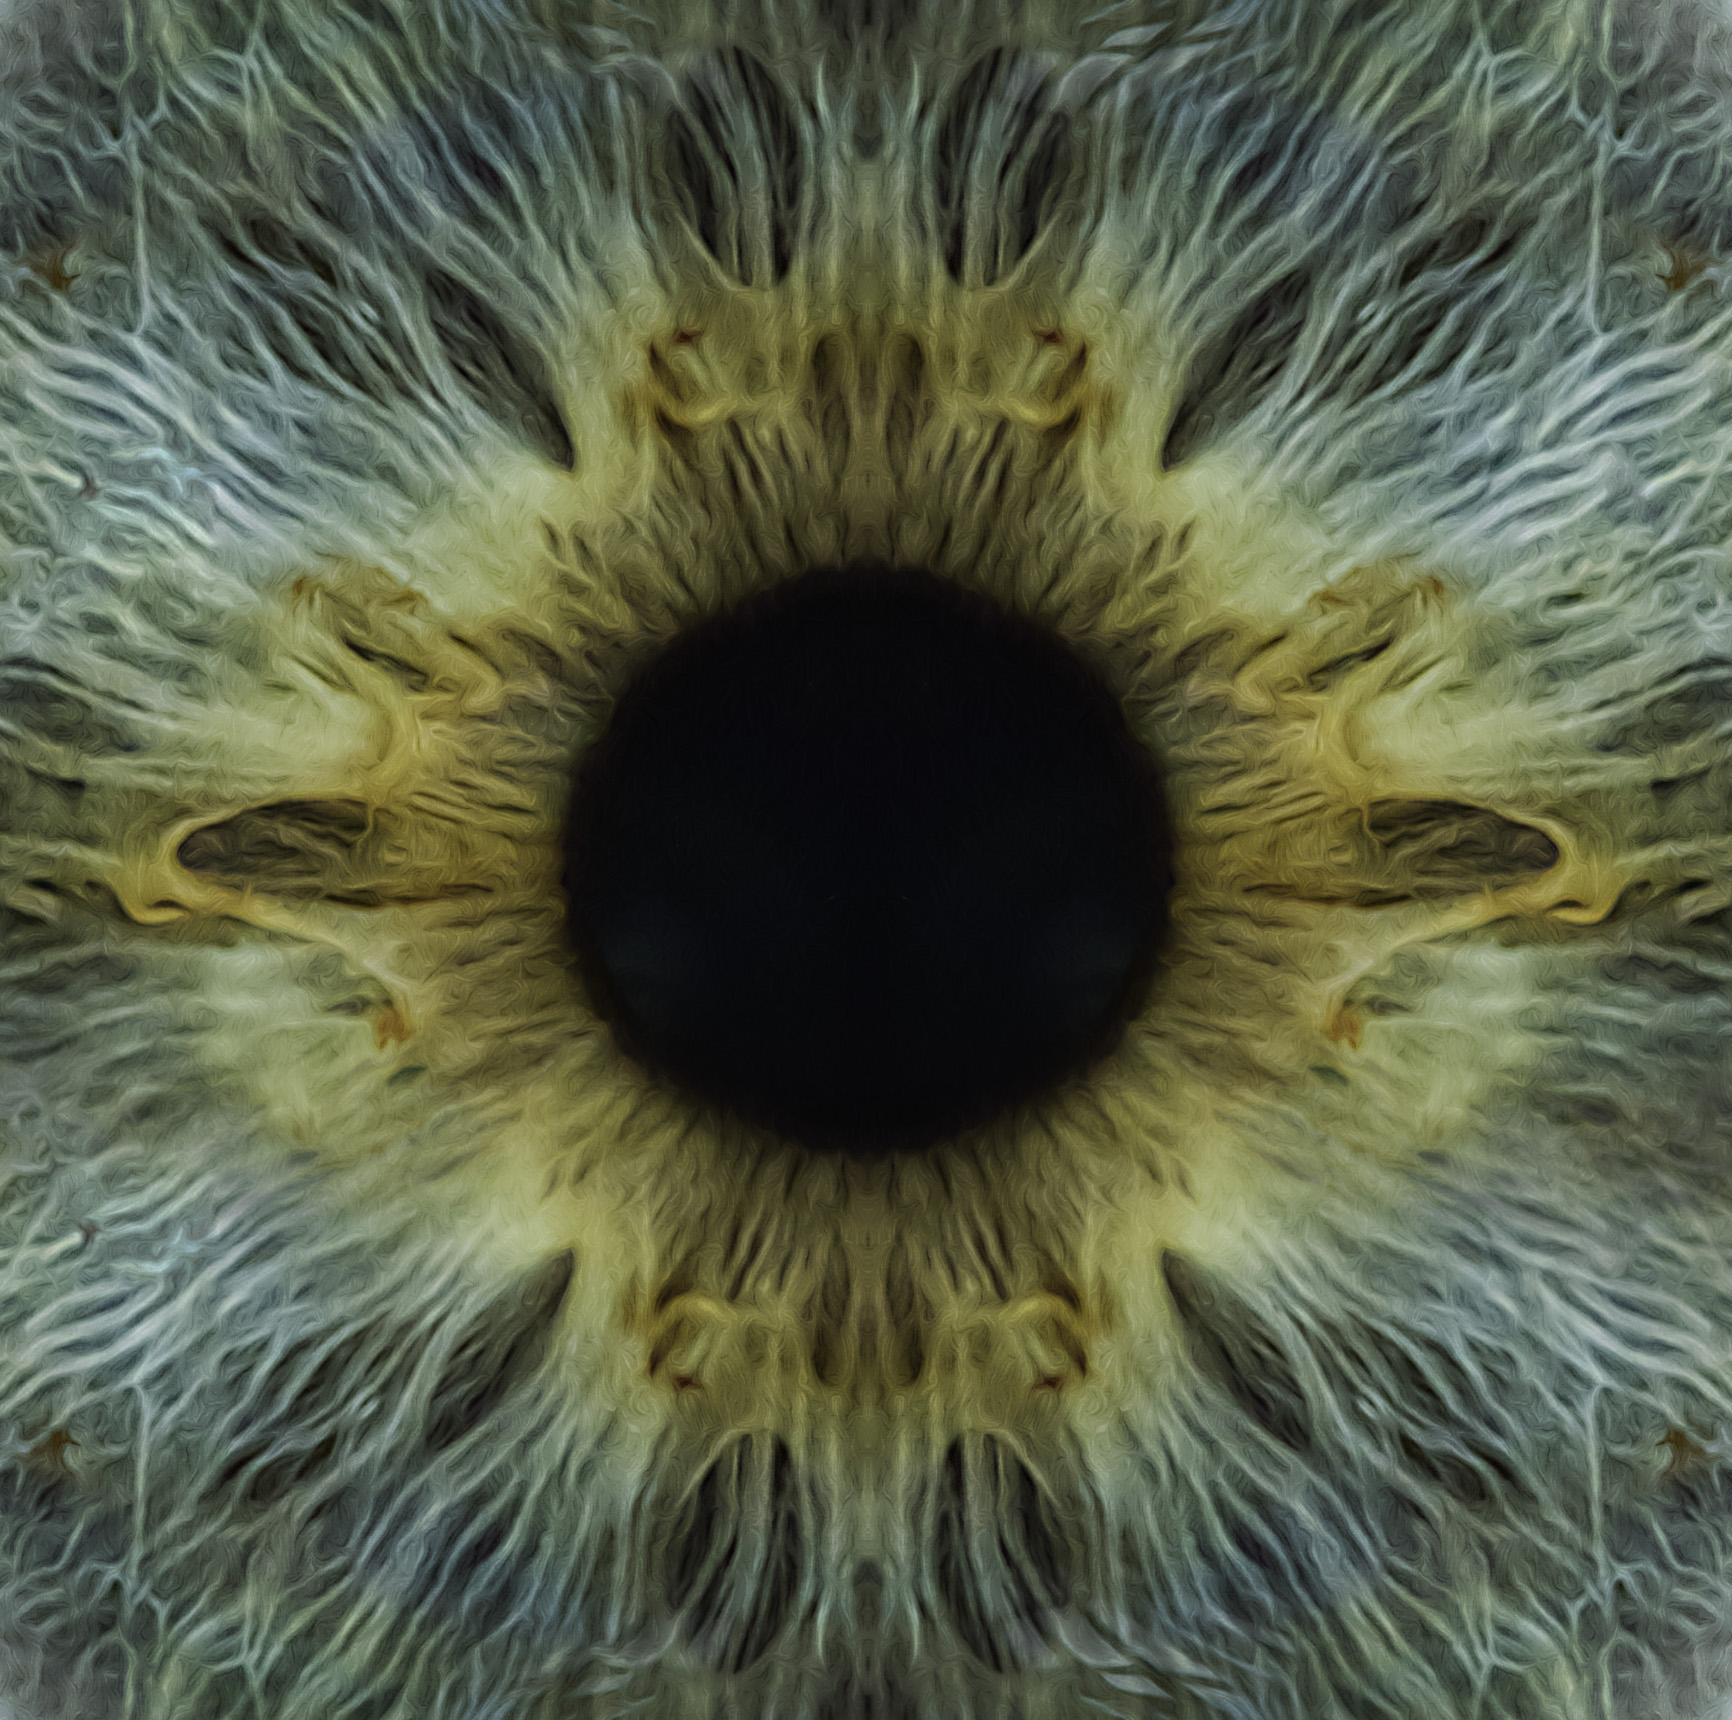
\includegraphics[width=0.60\textwidth]{iris_closeup.jpg}
    \caption{Macrofotografia ilustrativa da íris evidenciando o padrão radial de fibras, criptas e o
    colarete (faixa sinuosa que separa a zona pupilar da zona ciliar). Estas estruturas são alvo da
    caracterização morfológica proposta no Eixo~3. Crédito: Carlos Andrés Reyes, via Wikimedia Commons,
    licença CC~BY~2.0 (imagem com pós-processamento artístico; uso meramente ilustrativo).}
    \label{fig:iris-closeup}
\end{figure}

\subsection{Diabetes mellitus tipo 2 e o olho}
O DM2 é uma doença metabólica crônica de alta prevalência, associada a complicações micro e
macrovasculares \citep{WHOdiabetes2024}. A complicação ocular mais estudada é a retinopatia diabética,
mas a microangiopatia e a neuropatia autonômica também afetam o \textbf{segmento anterior}.
Esses efeitos mensuráveis na íris e na pupila fornecem a referência clínica utilizada neste trabalho,
sem recorrer a pressupostos iridológicos.

\subsection{Vascularização da íris no DM2}
Evidências com AS-OCTA indicam que a densidade vascular da íris é \textbf{reduzida} em pacientes com
DM2, inclusive na ausência de retinopatia diabética. \citet{Zhou2025SciRep} avaliaram a vasculatura
iridiana em pacientes com DM2 sem retinopatia e observaram redução significativa da densidade vascular
da íris (íris total e setores nasal e temporal), com associações a sexo, índice de massa corporal e
glicemia. Trabalhos metodológicos demonstram a viabilidade de identificar e estadiar a vasculatura da
íris por AS-OCTA \citep{Roberts2017CER} e de compará-la à angiofluoresceinografia \citep{Zett2018Graefes}.
Embora a AS-OCTA não esteja disponível em fotografias convencionais, esses estudos motivam a
investigação de correlatos texturais e cromáticos da vascularização em imagens RGB. Métodos de
aprendizado de máquina também foram aplicados à análise quantitativa de angiografias da íris
\citep{Zhu2026QIMS}.

\subsection{Diâmetro pupilar, espessura iridiana e disautonomia}
\citet{Cui2024BMC} estudaram a relação entre fluxo sanguíneo da íris, espessura iridiana e diâmetro
pupilar em repouso e após midríase farmacológica em diabéticos, encontrando, em adultos com DM2,
íris mais delgada na região do dilatador e \textbf{menor diâmetro pupilar} --- com a hemoglobina
glicada (HbA1c) atuando como fator independente do diâmetro pupilar após dilatação. De modo
convergente, \citet{Thakar2025Eye} reportam, por pupilometria automatizada, \textbf{diâmetros
pupilares significativamente menores} em diabéticos, com correlação a parâmetros de neurodegeneração
retiniana. Esses achados sustentam o \textbf{diâmetro pupilar e a dinâmica pupilar} como biomarcadores
candidatos, potencialmente estimáveis por visão computacional a partir da segmentação pupila/íris.

\subsection{Descritores cromáticos}
O projeto quantifica a cor da íris com momentos de cor (média, desvio-padrão e assimetria) e
histogramas regionais nos espaços HSV e LAB. Esses espaços separam componentes de luminância e
crominância e permitem testar se os descritores permanecem estáveis sob mudanças de iluminação e
contraste.

\subsection{Visão computacional e aprendizado profundo}
A normalização \emph{rubber sheet} \citep{Daugman2004} mapeia a região anelar da íris para coordenadas
polares (raio~$\times$~ângulo), facilitando a extração de descritores comparáveis entre amostras.
Sobre essa representação aplicam-se descritores clássicos --- intensidades de pixel, \emph{Local Binary
Patterns} \citep{Ojala2002LBP} e descritores de Haralick derivados da matriz de coocorrência
\citep{Haralick1973Texture}. Também são avaliadas arquiteturas de aprendizado profundo ---
ResNet \citep{He2016ResNet}, EfficientNet \citep{Tan2019EfficientNet} e \emph{Vision Transformers}
\citep{Dosovitskiy2021ViT} ---, ajustadas por \emph{transfer learning}
\citep{Pan2010TransferLearning}. A aplicação dessas técnicas à oftalmologia inclui a detecção de
retinopatia diabética em retinografias \citep{Gulshan2016JAMA}. Modelos com maior capacidade também
podem aprender atalhos relacionados à aquisição \citep{Zech2018}; por isso, a avaliação por pessoa
depende de identificadores reais.

% ====================== Trabalhos Relacionados ======================
\section{Trabalhos Relacionados}

A Tabela~\ref{tab:relacionados} reúne estudos sobre íris, segmento anterior e DM2. Os trabalhos
clínicos medem vascularização, diâmetro pupilar e espessura com equipamentos próprios para essas
grandezas. Eles servem como referência para avaliar quais correlatos podem ser obtidos de fotografias
convencionais e quais informações dependem de modalidades como AS-OCTA.

\begin{table}[H]
\centering
\caption{Trabalhos relacionados: biomarcadores médicos da íris/pupila no DM2 e métodos associados.}
\label{tab:relacionados}
\small
\setlength{\tabcolsep}{4pt}
\renewcommand{\arraystretch}{1.25}
\begin{tabularx}{\textwidth}{>{\raggedright\arraybackslash}p{0.16\textwidth}
>{\centering\arraybackslash}p{0.06\textwidth}
>{\raggedright\arraybackslash}X
>{\raggedright\arraybackslash}p{0.20\textwidth}}
\toprule
\textbf{Referência} & \textbf{Ano} & \textbf{Foco / biomarcador} & \textbf{Método} \\
\midrule
\citeauthor{Zhou2025SciRep} & 2025 & Densidade vascular da íris reduzida em DM2 sem retinopatia &
AS-OCTA; análise estatística por setores \\
\citeauthor{Cui2024BMC} & 2024 & Fluxo sanguíneo, espessura da íris e diâmetro pupilar (repouso e
pós-midríase) & OCTA + AS-OCT + pupilômetro \\
\citeauthor{Thakar2025Eye} & 2025 & Diâmetro pupilar menor em diabéticos; correlação com camada de
fibras nervosas & Pupilometria automatizada \\
\citeauthor{Roberts2017CER} & 2017 & Identificação e estadiamento da vasculatura/neovascularização da
íris & AS-OCTA (estudo piloto) \\
\citeauthor{Zett2018Graefes} & 2018 & Vasculatura da íris: comparação de modalidades & AS-OCTA
\emph{vs.} angiofluoresceinografia \\
\citeauthor{Zhu2026QIMS} & 2026 & Análise quantitativa de angiografia da íris & Aprendizado de máquina \\
\citeauthor{Surya2026PLoS} & 2026 & Predição de retinopatia diabética a partir de anormalidades
pupilares & ML (rede neural artificial) \\
\citeauthor{SamantAgarwal2018CMPB} & 2018 & \emph{Pipeline} de classificação de DM2 por imagens da íris
(linha de base de referência) & ROI + descritores + RF \\
\bottomrule
\end{tabularx}
\end{table}

\paragraph{Posicionamento deste PGC.}
O projeto utiliza as medidas descritas na literatura clínica como referência, mas trabalha com
fotografias RGB, e não com AS-OCTA. A análise inclui deduplicação, múltiplas métricas, testes de
robustez e particionamento por pessoa quando houver identificadores reais. A equivalência clínica das
medidas indiretas não é presumida, e a validação externa permanece necessária.

% ====================== Metodologia ======================
\section{Metodologia Proposta}

\subsection{Fluxo computacional de base}
O fluxo implementado é composto por:
(1)~segmentação de íris e pupila; (2)~normalização geométrica \emph{rubber sheet}; (3)~extração de
descritores (intensidades de pixel, LBP e Haralick); (4)~classificação (Regressão Logística, SVM,
\emph{Random Forest}, MLP e AdaBoost); e (5)~avaliação padronizada sob validação cruzada estratificada
por grupos. O particionamento só é considerado por pessoa quando os grupos correspondem a
identificadores reais. Os arquivos de saída registram as divisões, os parâmetros e as versões dos
pacotes utilizados, permitindo comparar cada extensão com a linha de base.

\subsection{Estudo de viabilidade: medidas oculares a partir de imagens RGB}
Antes das extensões de modelagem, conduz-se um estudo de viabilidade para estimar correlatos dos
biomarcadores médicos (Figura~\ref{fig:pipeline}):

\begin{itemize}
    \item \textbf{Diâmetro pupilar e coroa pupilar.} A partir da segmentação pupila/íris, estima-se o
    raio/diâmetro pupilar relativo (normalizado pelo diâmetro da íris, para mitigar variações de
    escala/câmera) e a \textbf{razão pupila/íris}. A borda pupilar é ajustada a uma circunferência e
    quantificam-se os desvios radiais (Eixo~3).
    \item \textbf{Correlatos de vascularização.} Investigam-se realces de estruturas finas (filtros do
    tipo Frangi/\emph{vesselness}, realce de cor nos canais vermelho e verde e descritores de textura)
    como medidas indiretas de densidade vascular. Fotografias RGB não substituem AS-OCTA; a análise
    mede a viabilidade e a estabilidade desses correlatos, sem afirmar equivalência clínica.
    \item \textbf{Morfologia iridiana.} Densidade de criptas, sulcos e ondulação do colarete são
    estimadas sobre a íris normalizada.
\end{itemize}

As segmentações são submetidas a controle de qualidade antes da normalização: a borda pupilar deve
estar contida na borda iridiana, a largura anular deve permanecer positiva em todo o domínio angular,
as fronteiras devem permanecer dentro da imagem e o escore mínimo de qualidade deve ser atendido.
Falhas são registradas e excluídas, sem substituição silenciosa de medidas.

\begin{figure}[H]
\centering
\resizebox{0.98\textwidth}{!}{%
\begin{tikzpicture}[
    node distance=0.55cm and 0.55cm,
    box/.style={draw, rounded corners, align=center, font=\footnotesize,
                minimum height=0.95cm, text width=2.7cm, fill=blue!4},
    feat/.style={draw, rounded corners, align=center, font=\scriptsize,
                 minimum height=0.8cm, text width=2.7cm, fill=green!6},
    arr/.style={-{Stealth[length=2mm]}, thick, gray!60!black}
]
\node[box] (img) {Imagem RGB\\da íris};
\node[box, right=of img] (seg) {Segmentação\\íris + pupila};
\node[box, right=of seg] (norm) {Normalização\\\emph{rubber sheet}};
\node[box, right=of norm] (split) {Grupos por pessoa\\(IDs reais)};

\node[feat, below=1.1cm of seg, xshift=-1.2cm] (med) {\textbf{Medidas oculares}\\diâmetro pupilar,
coroa, vasc.\ (\emph{proxy})};
\node[feat, right=of med] (classic) {\textbf{Clássicas}\\pixels, LBP, Haralick};
\node[feat, right=of classic] (chrom) {\textbf{Cromáticas}\\momentos, HSV/LAB};
\node[feat, right=of chrom] (deep) {\textbf{Profundas}\\ResNet, EfficientNet, ViT};

\node[box, below=1.1cm of classic, xshift=0.0cm, fill=orange!8, text width=3.2cm] (clf)
{Classificação\\(LR, SVM, RF, MLP, \emph{deep})};
\node[box, right=of clf, fill=orange!8, text width=3.4cm] (eval)
{Avaliação\\Acc, Sens, Esp, Prec, F1\\+ robustez};

\draw[arr] (img) -- (seg);
\draw[arr] (seg) -- (norm);
\draw[arr] (norm) -- (split);
\draw[arr] (seg.south) to[out=-90,in=90] (med.north);
\draw[arr] (norm.south) to[out=-90,in=90] (classic.north);
\draw[arr] (norm.south) to[out=-90,in=90] (chrom.north);
\draw[arr] (split.south) to[out=-90,in=90] (deep.north);
\draw[arr] (med.south) to[out=-90,in=90] (clf.north);
\draw[arr] (classic.south) -- (clf.north);
\draw[arr] (chrom.south) to[out=-90,in=90] (clf.north);
\draw[arr] (deep.south) to[out=-90,in=90] (eval.north);
\draw[arr] (clf) -- (eval);
\end{tikzpicture}
}%
\caption{Visão geral do fluxo proposto. O processamento de base (azul) alimenta quatro grupos de
descritores (verde), incluindo medidas oculares indiretas, e a avaliação dos classificadores
(laranja).}
\label{fig:pipeline}
\end{figure}

\subsection{Eixo 1 --- Base de trabalho e proveniência clínica}
O arquivo legado recebido contém 108 linhas reportadas como controle e 88 como diabetes, mas não
inclui identificadores reais, lateralidade, fonte do diagnóstico ou confirmação do subtipo DM2. A
auditoria removeu 73 cópias exatas, restando 123 imagens únicas (66 controles reportados e 57 casos
reportados como diabetes). Portanto, essa base não dispensa a recuperação de metadados nem permite
afirmar isolamento por pessoa. O protocolo definitivo exige um manifesto
com identificador real, lateralidade, rótulo binário e fonte do diagnóstico; todas as imagens do mesmo
indivíduo são mantidas no mesmo grupo.

Enquanto o manifesto clínico não estiver disponível, o arquivo legado é usado somente em uma análise
provisória, mediante autorização explícita na linha de comando. A Figura~\ref{fig:baseline-preliminar} resume a acurácia dos cinco
classificadores sobre o conjunto completo de descritores, em três sementes e cinco \textit{folds} por
semente. O melhor resultado nessa configuração foi do \emph{Random Forest} (acurácia média 0,829),
enquanto a melhor ablação foi AdaBoost com descritores clássicos (0,840). Esses valores demonstram a
execução do protocolo; não demonstram associação específica com DM2 nem
generalização entre pessoas reais. A validação em conjunto independente permanece necessária.
A publicação associada ao arquivo também foi retratada pelo IEEE
\citep{RetractionNotice2023}; por isso, o conjunto não é usado como evidência científica, e qualquer
uso futuro depende de esclarecimento com o custodiante dos dados sobre proveniência, licença,
consentimento e implicações da retratação.

\begin{figure}[H]
    \centering
    \begin{tikzpicture}
    \begin{axis}[
        width=0.92\textwidth,
        height=7.5cm,
        ybar=2pt,
        bar width=9pt,
        ylabel={Acurácia},
        xlabel={Classificador},
        ymin=0.55, ymax=1.0,
        ytick={0.55,0.60,0.65,0.70,0.75,0.80,0.85,0.90,0.95,1.0},
        yticklabel style={font=\scriptsize},
        symbolic x coords={AdaBoost, MLP, RF, SVM, LR},
        xtick=data,
        xticklabel style={font=\small},
        legend style={at={(0.5,1.18)}, anchor=north, legend columns=1, font=\small, draw=gray!50},
        grid=major,
        major grid style={gray!20},
        enlarge x limits=0.18,
        nodes near coords,
        nodes near coords style={font=\tiny, rotate=90, anchor=west, xshift=0pt, yshift=1pt},
        every node near coord/.append style={/pgf/number format/fixed, /pgf/number format/precision=2},
    ]
    \addplot[fill=green!50!black!40, draw=green!60!black] coordinates {
        (AdaBoost,0.8239) (MLP,0.7941) (RF,0.8293) (SVM,0.7811) (LR,0.7753)
    };
    \addlegendentry{Todos os descritores}
    \end{axis}
    \end{tikzpicture}
    \caption{Linha de base provisória sobre 123 imagens únicas do arquivo legado: acurácia
    média de cinco classificadores com todos os descritores, em três sementes e cinco \textit{folds}
    por semente. Os grupos são IDs sintéticos por linha, não identificadores reais de pessoa, e a
    classe positiva significa diabetes reportado, sem confirmação do subtipo DM2.}
    \label{fig:baseline-preliminar}
\end{figure}

\subsection{Eixo 2 --- Arquiteturas profundas}
Avaliam-se ResNet, EfficientNet e \emph{Vision Transformers} sob \emph{transfer learning} (pesos
pré-treinados em ImageNet), com ajuste fino das camadas superiores. O particionamento por pessoa será
aplicado quando houver identificadores reais. A comparação com a linha de base clássica verifica se
essas arquiteturas acrescentam informação ou apenas aumentam o sobreajuste.

\subsection{Eixo 3 --- Caracterização morfológica da íris e da coroa pupilar}
A morfologia é quantificada por \textbf{desvios em relação à circunferência ajustada}
(Figura~\ref{fig:morfologia}). Ajusta-se uma circunferência à borda pupilar (e à fronteira
entre íris e esclera) e mede-se, em cada ângulo~$\theta$, o desvio radial
$\delta(\theta) = r_{\text{borda}}(\theta) - r_{\text{circ}}(\theta)$. Estatísticas de $\delta(\theta)$
(amplitude, energia espectral, número de lóbulos) descrevem a regularidade da coroa pupilar e da borda
pupilar, relacionando-se ao tônus muscular e à inervação autonômica.

\begin{figure}[H]
\centering
\begin{tikzpicture}[scale=1.1]
    % iris outer boundary
    \draw[thick, blue!50!black, fill=blue!3] (0,0) circle (3cm);
    \node[blue!50!black, font=\scriptsize] at (2.25,2.25) {íris};
    % fitted circle for pupil (reference)
    \draw[dashed, gray!70] (0,0) circle (1.15cm);
    % actual pupil boundary (slightly irregular) — approx with a wavy closed curve
    \draw[thick, red!70!black, fill=gray!25]
        plot[smooth cycle, tension=0.8] coordinates {
        (1.18,0.05) (0.78,0.82) (0.05,1.22) (-0.82,0.80) (-1.20,0.02)
        (-0.80,-0.85) (0.02,-1.18) (0.86,-0.80) };
    \node[font=\scriptsize] at (0,0) {pupila};
    % radial deviation arrows
    \draw[-{Stealth[length=1.6mm]}, orange!80!black, thick] (0,0) -- (30:1.15);
    \node[gray!70!black, font=\tiny] at (30:1.45) {$r_{\text{circ}}$};
    \draw[-{Stealth[length=1.6mm]}, red!70!black, thick] (0,0) -- (60:1.22);
    \node[red!70!black, font=\tiny] at (62:1.55) {$r_{\text{borda}}(\theta)$};
    % collarette (corona) ring
    \draw[densely dotted, violet!70] (0,0) circle (1.9cm);
    \node[violet!70, font=\tiny] at (-118:2.15) {colarete (coroa)};
    % theta angle
    \draw[->, gray] (0.7,0) arc[start angle=0, end angle=30, radius=0.7];
    \node[gray, font=\tiny] at (15:0.92) {$\theta$};
\end{tikzpicture}
\caption{Esquema da caracterização morfológica (Eixo~3). A borda pupilar real (vermelho) é comparada a
uma circunferência ajustada (tracejada); o desvio radial
$\delta(\theta)=r_{\text{borda}}(\theta)-r_{\text{circ}}(\theta)$ e a geometria do colarete (pontilhado)
descrevem a regularidade da coroa pupilar.}
\label{fig:morfologia}
\end{figure}

\subsection{Eixo 4 --- Descritores cromáticos}
Sobre a íris normalizada, extraem-se \textbf{momentos de cor} (média, desvio-padrão e assimetria por
canal) e \textbf{histogramas regionais} nos espaços \textbf{HSV} e \textbf{LAB}, globalmente e por
setores. Avalia-se o ganho marginal desses descritores sobre os descritores clássicos, bem como sua
estabilidade sob transformações fotométricas (contraste/iluminação).

\subsection{Particionamento, métricas e robustez}
Mantêm-se os controles metodológicos de base: (i)~particionamento por pessoa como
salvaguarda contra vazamento por identidade, condicionado a identificadores reais;
(ii)~validação cruzada estratificada por grupos; (iii)~métricas
múltiplas --- acurácia, sensibilidade, especificidade, precisão e F1 ---, com média e desvio-padrão
entre \textit{folds}; e (iv)~testes de robustez (sementes, reamostragens e perturbações fotométricas).
Para as análises locais e de múltiplos descritores, adota-se cautela quanto a \textbf{múltiplas
comparações}, tratando achados locais como hipóteses candidatas a confirmação.

\subsection{Aspectos éticos e de tratamento de dados}
Por envolver imagens associadas a uma condição de saúde (DM2), o trabalho observa princípios de
integridade em pesquisa e de proteção de dados. Antes de qualquer divulgação, a proveniência, a
licença de uso, a anonimização e a base legal do conjunto devem ser documentadas. O arquivo legado
atual não contém informação suficiente para comprovar esses requisitos e, por isso, permanece restrito
à validação operacional local.
Não se realizam procedimentos clínicos nem se emitem diagnósticos individuais: os modelos são avaliados
exclusivamente em nível de pesquisa, com finalidade exploratória. Caso etapas futuras demandem a
aquisição de novas imagens em ambiente clínico, prevê-se a submissão a Comitê de Ética em Pesquisa
(CEP) e a obtenção de consentimento livre e esclarecido, em conformidade com a Resolução CNS
nº~466/2012 e com a Lei Geral de Proteção de Dados (LGPD, Lei nº~13.709/2018). Ressalta-se, ademais,
que a iridologia não constitui método diagnóstico reconhecido pela medicina, de modo que os resultados
deste trabalho não devem ser interpretados como validação de práticas iridológicas.

% ====================== Cronograma ======================
\section{Cronograma}

O projeto distribui-se entre PGC~I (planejamento, fundamentação e viabilidade) e PGC~II (extensões,
integração e redação final), conforme a Tabela~\ref{tab:cronograma}.

\begin{table}[H]
\centering
\caption{Cronograma previsto de atividades (PGC~I e PGC~II). Cada bloco $\bullet$ indica um mês de
atividade prevista.}
\label{tab:cronograma}
\small
\setlength{\tabcolsep}{4pt}
\renewcommand{\arraystretch}{1.25}
\resizebox{\textwidth}{!}{%
\begin{tabular}{>{\raggedright\arraybackslash}p{6.6cm} *{12}{c}}
\toprule
\multirow{2}{*}{\textbf{Atividade}} & \multicolumn{6}{c}{\textbf{PGC I}} & \multicolumn{6}{c}{\textbf{PGC II}} \\
\cmidrule(lr){2-7}\cmidrule(lr){8-13}
 & M1 & M2 & M3 & M4 & M5 & M6 & M7 & M8 & M9 & M10 & M11 & M12 \\
\midrule
Revisão médica e computacional            & $\bullet$ & $\bullet$ & $\bullet$ &           &           &           &           &           &           &            &            &            \\
Estudo de viabilidade (medidas oculares) &       & $\bullet$ & $\bullet$ & $\bullet$ &           &           &           &           &           &            &            &            \\
Consolidação do fluxo computacional &  &           & $\bullet$ & $\bullet$ & $\bullet$ &           &           &           &           &            &            &            \\
Eixo 3 --- Caracterização morfológica     &           &           &           & $\bullet$ & $\bullet$ & $\bullet$ &           &           &           &            &            &            \\
Eixo 4 --- Descritores cromáticos         &           &           &           &           & $\bullet$ & $\bullet$ & $\bullet$ &           &           &            &            &            \\
Relatório/Defesa de PGC I                 &           &           &           &           &           & $\bullet$ &           &           &           &            &            &            \\
Eixo 2 --- Arquiteturas profundas         &           &           &           &           &           &           & $\bullet$ & $\bullet$ & $\bullet$ &            &            &            \\
Eixo 1 --- Base de trabalho rotulada para DM2 &       &           &           &           &           &           &           & $\bullet$ & $\bullet$ & $\bullet$  &            &            \\
Análises de robustez e integração final   &           &           &           &           &           &           &           &           & $\bullet$ & $\bullet$  & $\bullet$  &            \\
Redação, revisão e defesa de PGC II       &           &           &           &           &           &           &           &           &           & $\bullet$  & $\bullet$  & $\bullet$  \\
\bottomrule
\end{tabular}%
}
\end{table}

% ====================== Resultados Esperados ======================
\section{Resultados Esperados e Contribuições}

O projeto tem caráter exploratório e prevê os seguintes resultados:
\begin{itemize}
    \item um \textbf{diagnóstico de viabilidade} sobre extrair correlatos de vascularização, diâmetro
    pupilar e morfologia iridiana de imagens RGB convencionais, com limites e incertezas explicitados;
    \item uma \textbf{reavaliação da base legada}, limitada aos rótulos reportados, com as medidas
    oculares, os novos descritores e os testes de robustez, seguida por uma avaliação clínica quando
    houver confirmação de DM2 e identificadores reais;
    \item uma \textbf{comparação} entre descritores clássicos, morfológicos, cromáticos e
    arquiteturas profundas, sob os mesmos \textit{folds} e, quando possível, particionamento por
    pessoa;
    \item um fluxo computacional que registra dados, parâmetros, divisões e resultados e que pode ser
    reaplicado quando uma base clinicamente verificável estiver disponível.
\end{itemize}

A principal contribuição é metodológica. O trabalho define como testar, sem pressupostos
iridológicos, se fotografias da íris contêm medidas associadas ao DM2. O protocolo explicita as
limitações da base legada, controla vazamento de dados e estabelece os dados necessários para uma
validação clínica posterior.

% ====================== Referências ======================
\newpage
\begin{thebibliography}{99}

\bibitem[Cui et~al.(2024)]{Cui2024BMC}
Cui, L.; Xiao, Y.; Xiang, Z.; Chen, Z.; Yang, C.; Zou, H.
\newblock Study on the correlation between iris blood flow, iris thickness and pupil diameter in the
resting state and after pharmacological mydriasis in patients with diabetes mellitus.
\newblock \emph{BMC Ophthalmology}, 24(1):52, 2024.
\newblock doi: 10.1186/s12886-024-03322-y.

\bibitem[Daugman(2004)]{Daugman2004}
Daugman, J.
\newblock How iris recognition works.
\newblock \emph{IEEE Transactions on Circuits and Systems for Video Technology}, 14(1):21--30, 2004.
\newblock doi: 10.1109/TCSVT.2003.818350.

\bibitem[Dosovitskiy et~al.(2021)]{Dosovitskiy2021ViT}
Dosovitskiy, A.; Beyer, L.; Kolesnikov, A.; Weissenborn, D.; Zhai, X.; Unterthiner, T.; Dehghani, M.;
Minderer, M.; Heigold, G.; Gelly, S.; Uszkoreit, J.; Houlsby, N.
\newblock An image is worth 16$\times$16 words: Transformers for image recognition at scale.
\newblock In: \emph{International Conference on Learning Representations (ICLR)}, 2021.

\bibitem[Ernst(2000)]{Ernst2000ArchOphthalmol}
Ernst, E.
\newblock Iridology: a systematic review.
\newblock \emph{Archives of Ophthalmology}, 118(1):120--121, 2000.

\bibitem[Gulshan et~al.(2016)]{Gulshan2016JAMA}
Gulshan, V.; Peng, L.; Coram, M.; et~al.
\newblock Development and validation of a deep learning algorithm for detection of diabetic
retinopathy in retinal fundus photographs.
\newblock \emph{JAMA}, 316(22):2402--2410, 2016.
\newblock doi: 10.1001/jama.2016.17216.

\bibitem[Haralick et~al.(1973)]{Haralick1973Texture}
Haralick, R. M.; Shanmugam, K.; Dinstein, I.
\newblock Textural features for image classification.
\newblock \emph{IEEE Transactions on Systems, Man, and Cybernetics}, 3(6):610--621, 1973.
\newblock doi: 10.1109/TSMC.1973.4309314.

\bibitem[He et~al.(2016)]{He2016ResNet}
He, K.; Zhang, X.; Ren, S.; Sun, J.
\newblock Deep residual learning for image recognition.
\newblock In: \emph{IEEE Conference on Computer Vision and Pattern Recognition (CVPR)}, p.
770--778, 2016.
\newblock doi: 10.1109/CVPR.2016.90.

\bibitem[Ojala et~al.(2002)]{Ojala2002LBP}
Ojala, T.; Pietik\"ainen, M.; M\"aenp\"a\"a, T.
\newblock Multiresolution gray-scale and rotation invariant texture classification with local binary
patterns.
\newblock \emph{IEEE Transactions on Pattern Analysis and Machine Intelligence}, 24(7):971--987, 2002.
\newblock doi: 10.1109/TPAMI.2002.1017623.

\bibitem[Pan e Yang(2010)]{Pan2010TransferLearning}
Pan, S. J.; Yang, Q.
\newblock A survey on transfer learning.
\newblock \emph{IEEE Transactions on Knowledge and Data Engineering}, 22(10):1345--1359, 2010.
\newblock doi: 10.1109/TKDE.2009.191.

\bibitem[Roberts et~al.(2017)]{Roberts2017CER}
Roberts, P. K.; Goldstein, D. A.; Fawzi, A. A.
\newblock Anterior segment optical coherence tomography angiography for identification of iris
vasculature and staging of iris neovascularization: a pilot study.
\newblock \emph{Current Eye Research}, 42(8):1136--1142, 2017.
\newblock doi: 10.1080/02713683.2017.1293113.

\bibitem[Samant e Agarwal(2018)]{SamantAgarwal2018CMPB}
Samant, P.; Agarwal, R.
\newblock Machine learning techniques for medical diagnosis of diabetes using iris images.
\newblock \emph{Computer Methods and Programs in Biomedicine}, 157:121--128, 2018.
\newblock doi: 10.1016/j.cmpb.2018.01.004.

\bibitem[IEEE(2023)]{RetractionNotice2023}
IEEE.
\newblock Retraction notice: Discovering informative regions in iris images to predict diabetes.
\newblock In: \emph{2018 25th National and 3rd International Iranian Conference on Biomedical
Engineering (ICBME)}, 2023.
\newblock doi: 10.1109/ICBME45317.2018.10207763.

\bibitem[Simon et~al.(1979)]{Simon1979JAMA}
Simon, A.; Worthen, D. M.; Mitas, J. A.
\newblock An evaluation of iridology.
\newblock \emph{JAMA}, 242(13):1385--1389, 1979.

\bibitem[Surya et~al.(2026)]{Surya2026PLoS}
Surya, J.; Tamilselvi, S.; Roy, M.; et~al.
\newblock Machine learning-based prediction of diabetic retinopathy from pupillary abnormalities in a
South Indian population.
\newblock \emph{PLoS ONE}, 21(1):e0340802, 2026.
\newblock doi: 10.1371/journal.pone.0340802.

\bibitem[Tan e Le(2019)]{Tan2019EfficientNet}
Tan, M.; Le, Q. V.
\newblock EfficientNet: Rethinking model scaling for convolutional neural networks.
\newblock In: \emph{International Conference on Machine Learning (ICML)}, p. 6105--6114, 2019.

\bibitem[Thakar et~al.(2025)]{Thakar2025Eye}
Thakar, M.; et~al.
\newblock Quantitative automated pupillometry in diabetic patients and correlation with retinal nerve
fibre layer thickness.
\newblock \emph{Eye (London)}, 39(10):1983--1989, 2025.
\newblock doi: 10.1038/s41433-025-03793-3.

\bibitem[WHO(2024)]{WHOdiabetes2024}
World Health Organization (WHO).
\newblock Diabetes (Fact sheet), 2024.
\newblock Disponível em: \url{https://www.who.int/news-room/fact-sheets/detail/diabetes}.

\bibitem[Zech et~al.(2018)]{Zech2018}
Zech, J. R.; Badgeley, M. A.; Liu, M.; Costa, A. B.; Titano, J. J.; Oermann, E. K.
\newblock Variable generalization performance of a deep learning model to detect pneumonia in chest
radiographs: A cross-sectional study.
\newblock \emph{PLOS Medicine}, 15(11):e1002683, 2018.
\newblock doi: 10.1371/journal.pmed.1002683.

\bibitem[Zett et~al.(2018)]{Zett2018Graefes}
Zett, C.; Stina, D. M. R.; Kato, R. T.; Novais, E. A.; Allemann, N.
\newblock Comparison of anterior segment optical coherence tomography angiography and fluorescein
angiography for iris vasculature analysis.
\newblock \emph{Graefe's Archive for Clinical and Experimental Ophthalmology}, 256(4):683--691, 2018.
\newblock doi: 10.1007/s00417-018-3935-7.

\bibitem[Zhou et~al.(2025)]{Zhou2025SciRep}
Zhou, Y.; Wang, T.; Guo, Z.; She, F.; Zeng, J.; Zhu, X.
\newblock Assessment of iris vasculature in type 2 diabetes mellitus patients without diabetic
retinopathy using anterior segment optical coherence tomography angiography.
\newblock \emph{Scientific Reports}, 15(1):19035, 2025.
\newblock doi: 10.1038/s41598-025-04463-w.

\bibitem[Zhu et~al.(2026)]{Zhu2026QIMS}
Zhu, Y.; Sun, S.; Han, S.; Chen, J.; Western, D.; Zhang, L.
\newblock Automated method for quantitative analysis of iris fluorescein angiography based on machine
learning.
\newblock \emph{Quantitative Imaging in Medicine and Surgery}, 16(1):68, 2026.
\newblock doi: 10.21037/qims-2025-480.

\end{thebibliography}

\end{document}
